\subsubsection{Caso d'uso UC8.1.10: Creazione domanda con area cliccabile nell'immagine}
\label{UC8.1.10}
\begin{figure}[h]
	\centering
	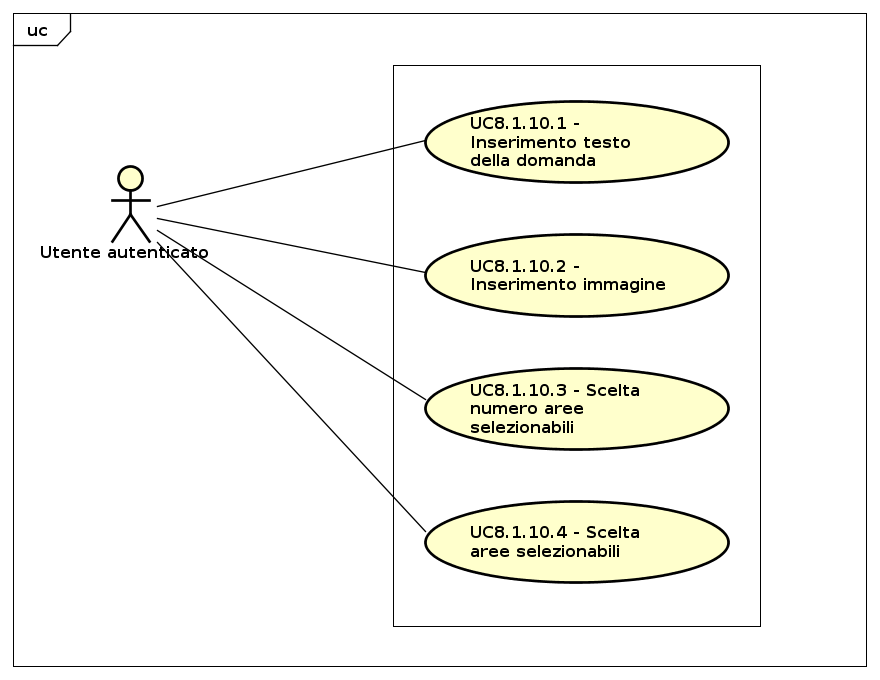
\includegraphics[scale=0.5,keepaspectratio]{UML/UC8_1_10.png}
	\caption{UC8.1.10: Creazione domanda con area cliccabile nell'immagine}
\end{figure}
\FloatBarrier
\begin{itemize}
	\item \textbf{Attori}: utente autenticato, utente autenticato pro;
	\item \textbf{Descrizione}: l'attore ha selezionato la funzionalità di creazione di una domanda la cui risposta è selezionabile all'interno di aree cliccabili in un'immagine;
	\item \textbf{Precondizione}: il sistema presenta all'attore la procedura guidata per la creazione di una domanda con area cliccabile nell'immagine;
	\item \textbf{Postcondizione}: l'attore ha creato una domanda con area cliccabile nell'immagine;
	\item \textbf{Scenario principale}:
		\begin{enumerate}
	       	\item L'attore può inserire il testo della domanda (UC8.1.10.1);
	        \item L'attore può inserire un'immagine relativa al testo della domanda (UC8.1.10.2);
		\item L'attore può scegliere quante aree saranno selezionabili all'interno dell'immagine \\(UC8.1.10.3);
		\item L'attore può scegliere quali aree saranno selezionabili all'interno dell'immagine \\(UC8.1.10.4).
	 	\end{enumerate}
\end{itemize}

\subsubsection{Caso d'uso UC8.1.10.1: Inserimento testo della domanda}
\begin{itemize}
	\item \textbf{Attori}: utente autenticato, utente autenticato pro;
	\item \textbf{Descrizione}: l'attore può inserire il testo della domanda che vuole creare;
	\item \textbf{Precondizione}: il sistema presenta all'attore lo spazio destinato all'inserimento del testo della domanda;
	\item \textbf{Postcondizione}: l'attore ha inserito il testo della domanda;
	\item \textbf{Scenario principale}: l'attore inserisce il testo della domanda. 
\end{itemize}

\subsubsection{Caso d'uso UC8.1.10.2: Inserimento immagine}
\begin{itemize}
	\item \textbf{Attori}: utente autenticato, utente autenticato pro;
	\item \textbf{Descrizione}: l'attore può inserire un'immagine relativa al testo della domanda;
	\item \textbf{Precondizione}: il sistema presenta all'attore la funzionalità di inserire un'immagine;
	\item \textbf{Postcondizione}: l'attore ha inserito un'immagine relativa al testo della domanda;
	\item \textbf{Scenario principale}: l'attore può eliminare l'immagine inserita (UC8.1.3.7.2.1).			
	\end{itemize}

\subsubsection{Caso d'uso UC8.1.10.3: Scelta numero aree selezionabili}
\begin{itemize}
	\item \textbf{Attori}: utente autenticato, utente autenticato pro;
	\item \textbf{Descrizione}: l'attore può scegliere il numero di aree selezionabili all'interno dell'immagine;
	\item \textbf{Precondizione}: il sistema presenta all'attore la funzionalità di scegliere il numero di aree selezionabili all'interno dell'immagine; 	
	\item \textbf{Postcondizione}: l'attore ha scelto il numero di aree selezionabili all'interno dell'immagine;
	\item \textbf{Scenario principale}: l'attore sceglie il numero di aree selezionabili all'interno dell'immagine. 	
\end{itemize}

\subsubsection{Caso d'uso UC8.1.10.4: Scelta aree selezionabili}
\begin{itemize}
	\item \textbf{Attori}: utente autenticato, utente autenticato pro;
	\item \textbf{Descrizione}: l'attore ha la possibilità di scegliere dove inserire le aree selezionabili all'interno dell'immagine;
	\item \textbf{Precondizione}: il sistema presenta all'attore la funzionalità di scegliere dove inserire le aree selezionabili all'interno dell'immagine; 	
	\item \textbf{Postcondizione}: l'attore ha scelto dove inserire le aree selezionabili all'interno dell'immagine;
	\item \textbf{Scenario principale}: l'attore sceglie dove inserire le aree selezionabili all'interno dell'immagine. 	
\end{itemize}

